%
% The first command in your LaTeX source must be the \documentclass command.
\documentclass[sigconf]{acmart}
\usepackage[T1]{fontenc}
\usepackage[utf8]{inputenc}
\usepackage{colortbl}
\usepackage{amssymb}
%
% defining the \BibTeX command - from Oren Patashnik's original BibTeX documentation.
\def\BibTeX{{\rm B\kern-.05em{\sc i\kern-.025em b}\kern-.08emT\kern-.1667em\lower.7ex\hbox{E}\kern-.125emX}}
   
% Rights management information.
% This information is sent to you when you complete the rights form.
% These commands have SAMPLE values in them; it is your responsibility as an author to replace
% the commands and values with those provided to you when you complete the rights form.
%
% These commands are for a PROCEEDINGS abstract or paper.
\copyrightyear{2019}
\acmYear{2019}
\setcopyright{acmlicensed}
\acmConference[PEARC19]{PEARC19: Practice and Experience in Advanced Research Computing}{July 28 -- August 01, 2019}{Chicago, IL}
%\acmBooktitle{Woodstock '18: ACM Symposium on Neural Gaze Detection, June 03--05, 2018, Woodstock, NY}
%\acmPrice{15.00}
%\acmDOI{10.1145/1122445.1122456}
%\acmISBN{978-1-4503-9999-9/18/06}

%
% These commands are for a JOURNAL article.
%\setcopyright{acmcopyright}
%\acmJournal{TOG}
%\acmYear{2018}\acmVolume{37}\acmNumber{4}\acmArticle{111}\acmMonth{8}
%\acmDOI{10.1145/1122445.1122456}


%
% Submission ID.
% Use this when submitting an article to a sponsored event. You'll receive a unique submission ID from the organizers
% of the event, and this ID should be used as the parameter to this command.
%\acmSubmissionID{123-A56-BU3}

%
% The majority of ACM publications use numbered citations and references. If you are preparing content for an event
% sponsored by ACM SIGGRAPH, you must use the "author year" style of citations and references. Uncommenting
% the next command will enable that style.
%\citestyle{acmauthoryear}

%
% end of the preamble, start of the body of the document source.
\begin{document}

%
% The "title" command has an optional parameter, allowing the author to define a "short title" to be used in page headers.
\title[A Unified Software Environment for Canada’s Advanced Computing Centers]{Providing a Unified Software Environment for Canada’s National Advanced Computing Centers}

%
% The "author" command and its associated commands are used to define the authors and their affiliations.
% Of note is the shared affiliation of the first two authors, and the "authornote" and "authornotemark" commands
% used to denote shared contribution to the research.
\author{Maxime Boissonneault}
\email{maxime.boissonneault@calculquebec.ca}
\affiliation{%
  \institution{Université Laval, Calcul Québec, Compute Canada}
  \streetaddress{2325 Rue de l'Université}
  \city{Québec}
  \state{Québec}
  \country{Canada}
  \postcode{G1V 0A6}
}
\author{Bart E. Oldeman}
\email{bart.oldeman@calculquebec.ca}
\affiliation{%
  \institution{McGill University, Calcul Québec, Compute Canada}
  \streetaddress{845 Rue Sherbrooke Ouest}
  \city{Montréal}
  \state{Québec}
  \country{Canada}
  \postcode{H3A 0G4}
}

\author{Ryan P. Taylor}
\email{rptaylor@uvic.ca}
\affiliation{%
  \institution{University of Victoria, WestGrid, Compute Canada}
  \streetaddress{3800 Finnerty Rd}
  \city{Victoria}
  \state{British Columbia}
  \country{Canada}
  \postcode{V8P 5C2}}

%
% By default, the full list of authors will be used in the page headers. Often, this list is too long, and will overlap
% other information printed in the page headers. This command allows the author to define a more concise list
% of authors' names for this purpose.
\renewcommand{\shortauthors}{Boissonneault, Oldeman and Taylor}

%
% The abstract is a short summary of the work to be presented in the article.
\begin{abstract}
Exploiting an advanced computing platform consisting of several clusters distributed across the second-largest country in the world is challenging. Each cluster may run a different operating system, use a different generation of CPU, GPU, or network fabric, or be managed by a different team of system administrators. Presenting a unified software environment can tremendously facilitate the task of supporting researchers, but is challenging to implement. This is nevertheless what Compute Canada set out to do in 2016, in the midst of deploying a new generation of large clusters. 

We had to find software solutions to solve the challenges involved to achieve this goal. Distribution, portability and performance were three important technical criteria for us. We also had to consider the practicality of each approach for our users, and reproducibility of software installations performed by staff located at various sites across Canada. 

In this paper, we present the solution that we created, which has allowed Compute Canada to serve the needs of over 10,000 researchers across the country. This solution is used on over 20 different clusters with heterogeneous configurations, on processor architectures ranging from AMD's 2010 Magny-Cours to Intel's 2017 Skylake SP, with or without GPUs, with InfiniBand, Ethernet or OmniPath as the network fabric, and with Slurm or Torque/Moab as the scheduler. This stack provides a unified software environment to users, providing over 600 different scientific applications that are available in over 4,000 different combinations of version, compiler and CPU architecture.
\end{abstract}

%
% The code below is generated by the tool at http://dl.acm.org/ccs.cfm.
% Please copy and paste the code instead of the example below.
%

%\ccsdesc[500]{Computer systems organization~Embedded systems}
%\ccsdesc[300]{Computer systems organization~Redundancy}
%\ccsdesc{Computer systems organization~Robotics}
%\ccsdesc[100]{Networks~Network reliability}

%
% Keywords. The author(s) should pick words that accurately describe the work being
% presented. Separate the keywords with commas.
\keywords{cvmfs, easybuild, nix, software deployment}

%
% A "teaser" image appears between the author and affiliation information and the body
% of the document, and typically spans the page.
%\begin{teaserfigure}
%  \includegraphics[width=\textwidth]{sampleteaser}
%  \caption{Seattle Mariners at Spring Training, 2010.}
%  \Description{Enjoying the baseball game from the third-base seats. Ichiro Suzuki preparing to bat.}
%  \label{fig:teaser}
%\end{teaserfigure}

%
% This command processes the author and affiliation and title information and builds
% the first part of the formatted document.
\maketitle

\section{Introduction}
\label{sec:Introduction}
In 2016, Compute Canada set out to refresh its advanced computing infrastructure by deploying a few large clusters to replace nearly 30 smaller legacy clusters. This was a good opportunity to rethink our approach to software installation. Up to this point, each of the legacy clusters required individual manual software installation. This was laborious because each software package had to be installed dozens of times, and it created a poor experience for users when moving between clusters, due to inconsistencies in software installations. When we set out to build a common software environment, we first established four guiding principles for our design choices.

The first principle is that software packages should be available on every cluster (unless not possible because of license or hardware reasons). This meant that we needed a scalable resilient multi-site distribution mechanism. There are a few solutions that could be used, and we will discuss them in Section~\ref{sec:Distribution_mechanism}. The solution we opted for is CERN Virtual Machine File System, or CVMFS\cite{CVMFS}.

The second principle is that the software environment should be decoupled from the underlying operating system. Since each tool for software package installation has different strengths and weaknesses, we adopted a layered approach to leverage the best tool in each situation. We briefly describe this in Section~\ref{sec:Layered_environment}.

When we first designed the solution, new clusters were being deployed with the CentOS 7 operating system. However, they did not all have the same set of system packages installed. Moreover, we were interested in supporting legacy clusters
that were running CentOS 6, and virtual machines launched by users on several Compute Canada cloud platforms. In order to use the unified software environment on all of these systems, we needed a compatibility layer. 
The solution we deployed is Nix \cite{Nix}, although we are experimenting with Gentoo Prefix \cite{Gentoo} as a replacement. We will discuss these options in Section~\ref{sec:Compatibility_layer}.

The third principle is that installation procedures should be tracked and reproducible. This means that automation is needed. Nix already addresses this issue; however it mostly targets basic Linux packages. For scientific packages, we also wanted to ensure that the software packages were optimized for specific hardware architectures, which Nix cannot do easily. The tool we chose for this task is EasyBuild~\cite{EasyBuild2012,EasyBuild2014,EasyBuild2016}, which we will discuss in Section~\ref{sec:Scientific_applications}.

The fourth principle is that the interface presented to users should be as familiar as possible, and remain manageable with a very large number of software packages installed. All of our clusters were using a system of environment modules \cite{Modules1991,Modules1996}. However, the traditional module systems become unwieldy at the scale of thousands of installed modules. Using a hierarchical module tree, which is possible in a newer implementation of environment modules called Lmod \cite{Lmod}, helps address this problem. We will discuss how our implementation meets the third and fourth principles in Section~\ref{sub:Compiled_software_packages}.

Finally, we describe in Section~\ref{sec:Making_it_available} how you can use our software stack on your computer or cluster, and summarize the benefits of our design in Section~\ref{sec:Conclusion}.

\section{Distribution mechanism}
\label{sec:Distribution_mechanism}
A shared file system such as NFS, Lustre, or GPFS can provide access to software packages on a single cluster. However, experience in the field of high performance computing shows that parallel file systems are often challenging to operate at scale in a reliable and performant manner, especially for the high rate of I/O operations per second caused by applications starting. In addition, a shared file system is a single point of failure for a cluster, which nearly all jobs rely on in order to run. An alternative for a single cluster is to install binary packages on each node, using a mechanism such as RPM. However, this can result in divergent configurations across nodes, may be limited by available space on the local disks, and requires an additional configuration management layer to keep the packages synchronized. 

For a national platform spanning multiple clusters, latency precludes a parallel file system from consideration, and the synchronization problem is compounded. The clusters could be synchronized by pulling or pushing changes with a tool such as \texttt{rsync}, but this would not be scalable; even a tool as efficient as \texttt{rsync} takes several hours to synchronize over 40 million files and directories. Moreover, this method of copying files is not transactional or atomic, so an additional indirection layer would be required to provide a complete solution.

We therefore chose to use CERN Virtual Machine File System (CVMFS) \cite{CVMFS,CVMFS2012}. CVMFS is a file system designed to distribute software packages to clusters at a global scale with no single point of failure. Clients access files by pulling content on demand, using multiple levels of caching, to minimize network traffic and storage use and ensure responsive and scalable performance.

We will describe the general architecture of a CVMFS deployment in Section~\ref{sub:CVMFS_structure}, and describe the deployment specific to Compute Canada in Section~\ref{sub:CVMFS_in_CC}

\subsection{CVMFS architecture}
\label{sub:CVMFS_structure}
CVMFS is designed similarly to the Network Time Protocol stratum model, as illustrated in Figure~\ref{fig:CVMFS_structure}. There is one source of truth, the stratum 0 server, where software is published.  The stratum 0 is never accessed directly by clients. If it fails, the only immediate consequence is that publishing new files is not possible until it is back online. 

Snapshots of the software repositories on the stratum 0 are kept for a while, making it possible to roll back to a previous version if needed. Internally, CVMFS uses a content-addressable storage scheme, wherein files exceeding a certain size are broken into smaller objects, and each object is hashed, compressed, and stored in a location defined by its hash, resulting in automatic deduplication. Hashes also allow CVMFS clients to quickly verify the integrity of content received over the network, and quickly switch their repositories to new revisions when updates are published,  by means of a Merkle tree.

Data is replicated from the stratum 0 to multiple stratum 1 servers, which in turn serve content to clients via HTTP and provide redundancy and load balancing. Each cluster has local caching proxy servers to reduce the load placed on the stratum 1 servers by its compute nodes, accelerate access to any content missing from the local cache of a compute node, and mitigate the impact of a wide area network outage. The closest layer of cache can be configured to use a local disk on a node, or a shared file system in a diskless environment. Clients can also be configured to use two levels of cache together in a tiered manner, such as a solid state drive and a hard drive, or a hard drive and a shared file system.

\begin{figure}
  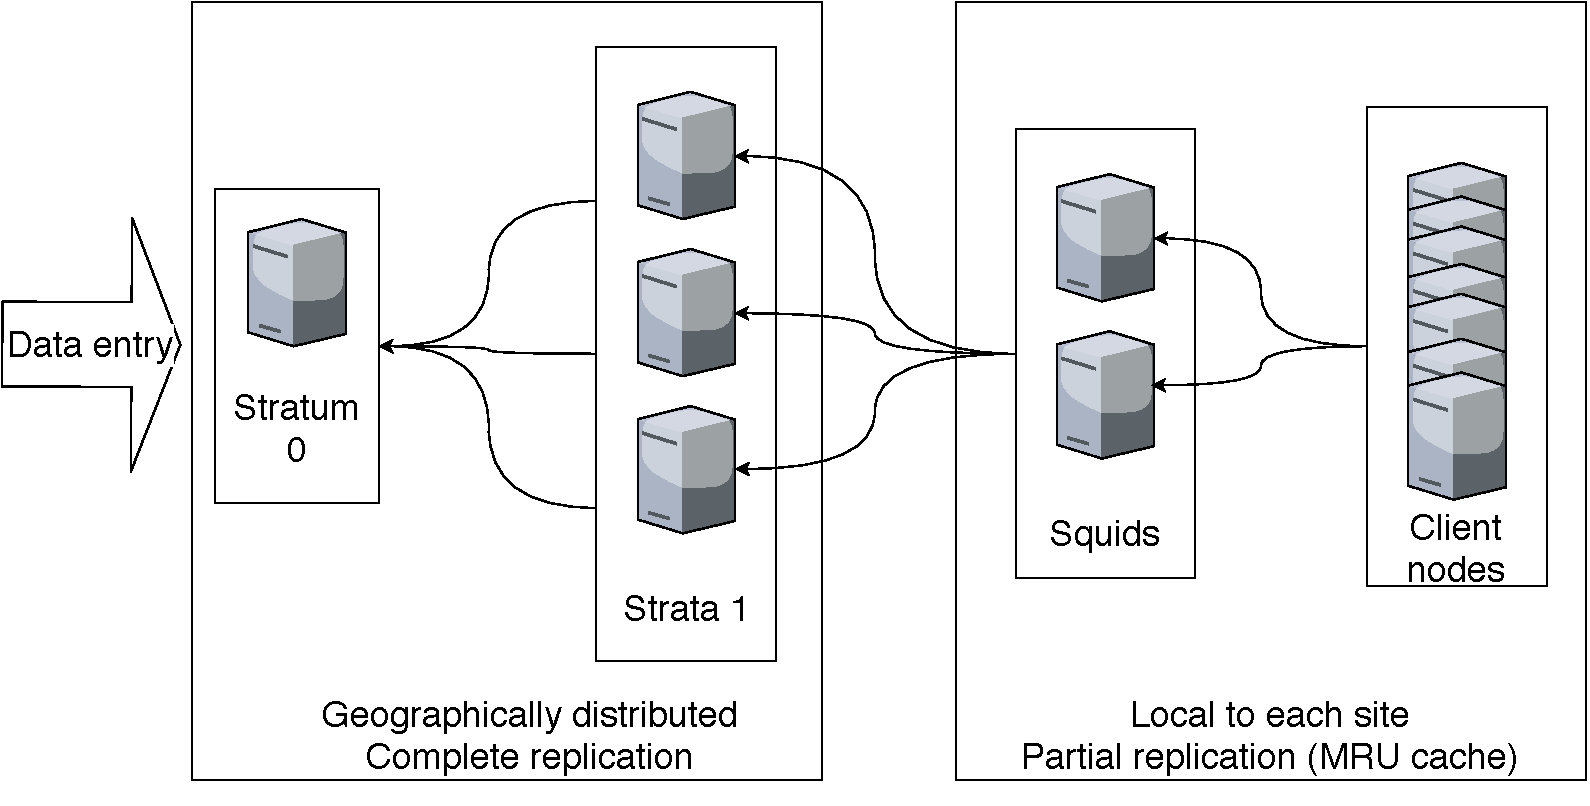
\includegraphics[width=0.45\textwidth]{CVMFS-structure.pdf}
  \caption{Diagram of the architecture of CVMFS. Arrows represent the flow of data. Data is pushed to the stratum 0, but is then fetched by the following layers.}
  \label{fig:CVMFS_structure}
\end{figure}

\subsection{Deployment of CVMFS in Compute Canada}
\label{sub:CVMFS_in_CC}
For Compute Canada's needs, we deployed two CVMFS server stacks, one for development and one for production, each of which is composed of a stratum 0 server and one or more stratum 1 servers. This allows us to follow a workflow that includes testing software packages before exposing them to users, as illustrated in Fig~\ref{fig:Workflow}. In total, three software repositories are used.

First, we have a development repository, hosted on the development servers. This repository is used to deploy software from our build infrastructure to the clusters without exposing it to end users. This allows us to test newly installed software packages on our clusters without impacting production, minimizing the risk of a faulty package causing problems for users. This is especially important, for example, when testing updates to software packages to fix bugs, or to make minor changes to an MPI implementation in order to correctly support a new cluster with a different networking fabric. 

We also have a production repository, hosted on the production servers. By design, software packages are always copied to the production repository from the development repository, and never directly from the build infrastructure. This step also minimizes the risk of faulty software affecting end users. This repository holds the software environment which is visible to the end users on all of our clusters. Once software is published to this repository, it becomes visible on all clusters within about 10 minutes. 

Both repositories above are available publicly, and can be mounted on any cluster or virtual machine in the cloud. There is a third repository, also hosted on the production servers, which provides software packages that are restricted to Compute Canada due to license limitations. We work with software vendors and developers in order to get the authorization to install licensed and commercial software packages in this repository. The most common licensing model that we use is a BYOL (bring your own license) model, in which we provide the software package, but end users provide a license server to connect to. Another model is to control access to a software package via POSIX groups. By default, the repository content on a CVMFS client belongs to a \texttt{cvmfs} service account and group, but this can be changed so that the original ownership metadata as published on the stratum 0 is used, thereby only allowing access to members of authorized POSIX groups. Since this relies on a specific LDAP domain and client configuration, access to this repository is restricted by network ACLs on the stratum 1 servers, and can only be granted to clusters that are run by Compute Canada teams. 

There is a fourth CVMFS repository that distributes configuration files instead of software. This special configuration repository resembles \texttt{/etc/cvmfs/} and provides information (such as URLs and public keys) required by CVMFS clients in order to access all {\it other} repositories. The benefit of this approach is that most CVMFS configuration can be centrally managed, and updates can be immediately pushed to all clients in order to set up a new repository or commission or decommission a stratum 1 server, rather than having to wait for all clients across the country to be updated.

One additional use case for CVMFS is to distribute datasets. By default, CVMFS  is optimized for a large number of small files, rather than a small number of large files, so different configurations and access methods are needed for data repositories. At the time of writing this paper, data repositories are used by some of our research groups in genomics, but not directly by our staff yet. 

\begin{figure}
  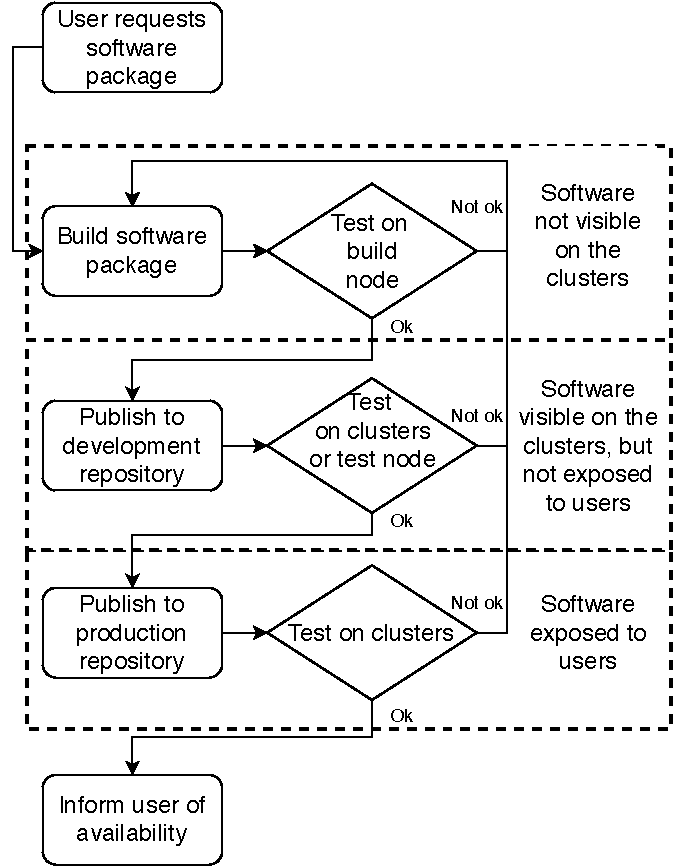
\includegraphics[width=0.45\textwidth]{Software-installation-workflow.pdf}
  \caption{Workflow followed by our software installers. At each step, there is a checkpoint to test if the software package works properly.}
  \label{fig:Workflow}
\end{figure}

\section{A layered approach}
\label{sec:Layered_environment}
To install software packages for our common environment, we follow a layered approach, as illustrated in Table~\ref{tab:layers}. First, we require a basic Linux installation. Any version of Linux with a kernel 2.6.32 (as used by RHEL 6 and its derivatives) or more recent should work. This layer is managed by the system administrators, and contains all drivers, typically provided by kernel modules and closely associated libraries, such as GPU and network drivers, as well as privileged binaries. 

The second and third layers constitute what we call our compatibility layer, containing almost all packages that one would typically install with the Linux distribution's package manager, such as \texttt{yum} or \texttt{apt-get}. 

The fourth and fifth layers are the scientific application layers. They contain mostly scientific or performance critical applications, including for example MPI implementations, the CUDA toolkit, mathematical libraries, and domain specific applications. 

\begin{table*}
  \begin{center}
  {\Large
  \begin{tabular}{|p{0.7\textwidth}|}
  \hline \cellcolor{cyan}
  EasyBuild layer: modules for Intel, PGI, Open MPI, MKL, high-level applications.
  Multiple instruction sets (SSE3, AVX, AVX2, AVX512).\newline
  \texttt{/cvmfs/soft.computecanada.ca/easybuild/\{modules,software\}/2017}\\
  \hline \cellcolor{green}
  EasyBuild-generated modules around Nix profiles: for example Clang, Eclipse,
  Erlang, FPC, GCC, Ruby.\newline
  \texttt{/cvmfs/soft.computecanada.ca/nix/var/nix/profiles/[a-z]\**}\\
  \hline \cellcolor{yellow}
  Nix layer: GNU C Library (glibc), autotools, make, bash, cat, ls, awk, grep, etc. \newline
  \texttt{module load nixpkgs/16.09 $\Rightarrow$ \$EBROOTNIXPKGS=} \newline
  \texttt{/cvmfs/soft.computecanada.ca/nix/var/nix/profiles/16.09}\\
  \hline \cellcolor{lightgray} 
  Gray area: Lustre client libraries, IB/OmniPath/InfiniPath client libraries 
  (all dependencies of Open MPI). In Nix layer, but can be overridden using
  \texttt{PATH} and \texttt{LD\_LIBRARY\_PATH}.\\
  \hline \cellcolor{pink}
  OS kernel, daemons, drivers, libcuda, anything privileged (e.g. the sudo
  command): always local. Some legally restricted software too, such as VASP.\\
  \hline
  \end{tabular}
  }
  \end{center}
  \caption{Layered structure of our software stack. The bottom layer (pink) is entirely managed by the system administrators of each cluster and is not on CVMFS. The second layer (grey) contains libraries that are available via Nix on CVMFS, but can be overridden locally. The third layer (yellow) contains everything that one would typically find in the Linux user space. The fourth layer (green) contains packages that you would typically find in an operating system, but for which multiple versions are required. They are installed through Nix, but wrapped into a module by EasyBuild. The top layer (cyan) contains packages that are not typically installed in a Linux distribution, and are installed via EasyBuild.}
  \label{tab:layers}
\end{table*}

\section{Compatibility layer}
\label{sec:Compatibility_layer}
Isolating the software environment from the operating system requires a compatibility layer containing almost everything that an OS would provide. We exclude the Linux kernel and its modules, hardware drivers, and privileged binaries from this layer. However, some libraries such as InfiniBand client libraries that are close to the hardware are also available in this layer (the gray area in Table~\ref{tab:layers}) and can optionally be used, or can be provided locally outside CVMFS.

\subsection{Nix}
\label{sub:Nix}
Nix~\cite{Nix} is both a package manager and an operating system (NixOS). One of the core principles in Nix is reproducibility, so it is designed to depend as little as possible on the underlying operating system. 

The installation path of each software package installed through Nix resides in a path called the Nix store. This store contains a single directory for each version of each software package installed through Nix. These directories are named after a hash calculated from the installation recipe and its dependencies. This creates a very large number of subdirectories, many of which contain nearly identical files. 

In addition to the store, Nix creates directories that are called profiles. These profile directories contain a forest of symbolic links that point to files in the Nix store. For example, each profile contains a \texttt{bin/} directory, which contains symbolic links to typical operating system commands such as \texttt{ls} and \texttt{gcc}, which reside in different paths in the store. A profile directory also contains \texttt{lib/} and \texttt{include/} directories which contain symbolic links to libraries and header files located in the store. We provide one main profile as the compatibility layer and some custom profiles for applications from that layer for which we provide multiple versions via modules that are generated by EasyBuild. Those custom profiles hence provide a hybrid between the top layer and the compatibility layer.

Profiles are the paths that are exposed to the end users, which is done by adding paths to their \texttt{PATH}, \texttt{CPATH} and other similar environment variables. Each profile ever created is kept, but users are only exposed to the most recent one. Each profile represents the complete state of the user-accessible environment at a given time.

Nix has a mechanism for garbage collection, which can be used to delete packages that are no longer used in the current profile. It also has a mechanism to resolve the complete list of files from the Nix store that are required to compose a given profile. Because Nix generates so many files, we use this mechanism to deploy on CVMFS only those files that are used in the current profile. 

This works well until a software package exposes paths to the Nix store directly, instead of the paths to Nix profiles. We call this a Nix store leak. This happens for example with Python when using virtual environments. Virtual environments in Python copy the \texttt{python} executable to a secondary location, outside of Nix. However, all binaries installed by Nix use \texttt{RPATH} for shared object resolution directly in the store. This means that copying a binary outside of Nix creates a dependency between a binary that now resides outside of the store, and the store itself. Because Nix is unaware of that dependency, any update of one of the dependencies followed by garbage collection or selective deployment of files will end up breaking this binary. We have encountered this issue with Python, Perl and Qt, which we have therefore moved outside of Nix and installed through EasyBuild instead.

Also, we have found that many Nix recipes call for installing sub-packages of a package in separate directories. For example, for Qt, \texttt{qmake} and \texttt{qtpaths} or \texttt{qtdiag} reside in different directories in the Nix store. This sometimes causes issues when installing a dependent package which assumes that its dependencies are installed in a more traditional fashion, with all of the binaries in the same \texttt{bin/} directory, alongside headers in the \texttt{include/} directory and libraries in the \texttt{lib/} directory.

In general, Nix provides an environment that is internally consistent but is best developed using Nix itself, through tools such as \texttt{nix-shell}. Such tools can only be used if the Nix store is writable, an impossibility with CVMFS. Attempting to use Nix in conjunction with other development tools using environment variables can be fragile at times. Moreover, the dependency of the hash on the whole installation recipe, instead of only the dependencies (as, for example, implemented in Spack~\cite{Spack}), causes the store path to change even if a bug fix or security update needs to be applied, aggravating this problem. We must note however, that some clusters in Compute Canada provide Nix with a writable Nix store, which is completely separate from the software stack described here.

\subsection{Gentoo Prefix}
\label{sub:Gentoo_Prefix}
Gentoo Prefix~\cite{Gentoo} is an alternative solution to provide a compatibility layer. It allows installation of most packages that form a typical Linux operating system, in a non-default location. Contrary to Nix however, packages are installed in a standard directory structure (\texttt{bin/}, \texttt{lib/}, \texttt{include/}, \texttt{share/}). This is helpful when updates are required, and minimizes problems with applications that expect a standard directory structure. At the time of this writing, we are still experimenting with Gentoo Prefix, and it is not used in production. 

\section{Scientific applications}
\label{sec:Scientific_applications}

\subsection{Compiled software packages}
\label{sub:Compiled_software_packages}
Scientific applications constitute the majority of our software stack. Since their performance is critical, they can not be installed in the compatibility layer, as they need to be optimized for specific CPU instruction sets. To install them, we use the EasyBuild~\cite{EasyBuild2012,EasyBuild2014,EasyBuild2016} software installation tool.

EasyBuild originated from the University of Ghent, but now has over 200 contributors from around the world. The framework is based on scripted recipes (in Python) to install packages, usually from source code. It is designed to create optimized binaries, and eases recompilation of multiple versions of a given application using many combinations of compilers or libraries. EasyBuild is composed of three parts: the framework, easyblocks, and easyconfig files (also known as ``easyconfigs''). 

The framework contains the core code which drives the logic of the entire software installation process, including parsing the configuration options, downloading source files, patching them, configuring, building and installing the software, as well as performing post-installation steps such as sanity checks, generating a module or running custom commands. 

Easyblocks are Python classes that define the steps required to install a given software package. There are generic easyblocks, such as \texttt{ConfigureMake} or \texttt{CMakeMake}, as well as custom easyblocks for packages that have more complicated installation procedures, such as OpenFOAM or PETSc. 

Easyconfig files parameterize the execution of the code from the easyblocks. They define the software name and version, the URL from which the source files can be downloaded, and options to be used for the various steps. 

In most cases, there is already an easyblock for a given software package, or it can be installed easily with one of the generic easyblocks. In these cases, writing a new recipe is as simple as editing a configuration file. EasyBuild also supports command line options to reuse an existing easyconfig file, while changing the software version or the toolchain being used. 

Toolchains are a core concept in EasyBuild. They represent a set or subset of a compiler, an MPI implementation, mathematical libraries and CUDA. Having the ability to generate multiple builds of a given software simply by providing a command line argument to change the toolchain has proven invaluable to our workflow, and has allowed us to recompile hundreds of packages in a matter of days when deploying a new version of compiler or a cluster with a new CPU architecture. 

EasyBuild also automatically creates module files~\cite{Modules1991,Modules1996,Lmod}. The framework supports multiple standard and custom naming schemes. We use a version of a hierarchical naming scheme, in which modules are organized in a tree structure, hiding those that are incompatible with currently loaded modules. This limits the list of visible modules, which could otherwise be very extensive. This can however confuse some users, since they don’t automatically see all available modules. Lmod~\cite{Lmod} alleviates this issue by providing a separate command to crawl the full module tree and instructs users on how to load the module they want.

\subsection{Handling multiple CPU architectures}
\label{sub:Handling_multiple_CPU_architectures}
Handling multiple CPU architectures is done by installing applications in architecture-dependent paths and module trees. We also have a wide selection of software packages that are installed in an architecture-independent fashion. This is the case, for example, for binary packages, packages that are not performance critical, or packages that consist of source files only. The same recipe is typically used for installing the same package for multiple architectures. While each cluster will usually show only a single architecture, users are allowed to select a different architecture if they wish to run exactly the same binary as on another cluster.

\subsection{Packages for scripting languages}
\label{sub:Packages_for_scripting_languages}
For scripting languages that support installing packages, such as Python, R or Perl, we leverage the existing package manager of that language, rather than installing them as modules. In the case of Python, we build Python wheels~\cite{Wheels}, linked against our software stack. Wheels are binary packages that can be installed in a matter of seconds, similar to RPM packages. Since they are built by our team, and linked against our optimized software stack, we ensure that they are easy to install and offer good performance.

\subsection{Documentation of supported packages}
\label{sub:Documentation}
Every software package that is installed through EasyBuild gets automatically listed on our documentation website:
\begin{center}
    \url{https://docs.computecanada.ca/wiki/Available_software}
\end{center}
Similarly, a list of available Python wheels is automatically generated:
\begin{center}
\url{https://docs.computecanada.ca/wiki/Available_wheels}    
\end{center}

\subsection{Logging of module usage}
\label{sub:Logging}
Our module system will automatically log (through \texttt{logger}) each module that is loaded. The information is logged in an easily parsable list of key-value pairs, which can then be aggregated into your favorite monitoring tool, such as Elastic Search. 

\section{Making the software environment available on your system}
\label{sec:Making_it_available}
To access the Compute Canada repositories on your own computer, you can install and configure the CVMFS client as described here:
\begin{center}
    \url{https://docs.computecanada.ca/wiki/Accessing_CVMFS}
\end{center}

Then, to set up the Compute Canada software environment, simply execute this command: 

\begin{center}
\texttt{source \textbackslash \linebreak
/cvmfs/soft.computecanada.ca/config/profile/bash.sh}
\end{center}

If you plan to use our CVMFS repositories on a large number of nodes such as a cluster, or to present our software environment to your users, we ask that you first contact us as described in the documentation web page above. Also, if you set up a large number of client nodes we require that you deploy them behind one or more caching HTTP proxies, to avoid overloading the stratum 1 servers. Note that this software stack is provided as is and comes with absolutely no warranty. 

The default set of modules will automatically try to detect the most recent set of instructions that is supported by the CPU amongst  SSE3, AVX, AVX2 and AVX512. It will also try to detect whether the hardware has a Mellanox InfiniBand, Intel OmniPath, or Ethernet network fabric. If these are not detected correctly, or if you have a cluster made up of mixed hardware, you can overwrite these defaults by defining the \texttt{RSNT\_ARCH} or \texttt{RSNT\_INTERCONNECT} environment variables before executing the command above. 

Note that the first time any software or data is accessed, it will take longer to load, as the CVMFS client is fetching the content from our stratum 1 servers. However, subsequent access will be much faster once the content is cached locally. 
Also note that the command above will {\it not} import our environment for any user IDs lower than 1000, which are typically privileged users on a Linux system. In order to force the command above to execute nevertheless, you can create a file named \texttt{.force\_cc\_cvmfs} in the user's \texttt{\$HOME} directory. Conversely, a \texttt{\$HOME/.skip\_cc\_cvmfs} file can be created to exclude a user from setting up the software environment. This is recommended for system administrators so their environment does not depend on CVMFS, especially if they are doing operations which may interrupt access to CVMFS, such as updating or reconfiguring it.


\section{Conclusion}
\label{sec:Conclusion}
We have built a software environment that is portable, is optimized for multiple CPU architectures and network interconnects, and can be deployed in a matter of minutes on a single node, and not much longer for a whole cluster. The design of the infrastructure guarantees that the software environment seen by our end users is the same across all of our clusters, and will not diverge over time. This makes it much easier for users to use multiple clusters or migrate between clusters, improving the user experience. It also reduces the workload on our staff by unifying the installation process for all clusters, and makes supporting our users easier because all clusters work the same way.

Because of the portability of our software stack and the distribution mechanism, it can be used on any cluster, or any Linux computer or virtual machine on a cloud. For example, for training events, we have been using it to provision small replicas of Compute Canada clusters in short-lived virtual clusters deployed on our OpenStack platform. We have also used this portable software environment to expose a cluster environment directly through a browser, via JupyterHub. 

Since software installation is no longer tightly coupled to any particular site or system, this approach has reduced the time required to commission major new Compute Canada clusters and make them accessible to our users by several months. At the same time, it also benefits universities and other research organizations running smaller or older clusters, desktops, and laboratory computing infrastructure, which may not have the human resources to build and maintain a comprehensive research software stack.


\section{Acknowledgments}
\label{sec:Acknowledgments}
We thank the following organizations and individuals for sharing their time and expertise:
\begin{itemize}
	\item All of the Compute Canada team members who make it possible to manage such a large software stack
	\item Robert McLay, from Texas Advanced Computing Center, for always providing quick and efficient support and
debugging for Lmod
	\item Kenneth Hoste from Ghent University, and Åke Sandgren from Umeå University, for many discussions
regarding EasyBuild
    \item All of the EasyBuild maintainers and contributors, without which EasyBuild would not have nearly as many supported recipes.
	\item Kuang Chung Chen and Bryan Caron, from McGill University, for initiating the groundwork in Compute Canada that lead to this project
	\item Dave Dykstra, Jakob Blomer, and the CernVM project team for support and development of CVMFS
\end{itemize}

% The next two lines define the bibliography style to be used, and the bibliography file.
\bibliographystyle{ACM-Reference-Format}
\bibliography{biblio}

\end{document}
